%\section{Secondary Measurement}
In this section we learn a macro usage which you may often encounter in actual situations: 
We do certain measurement first. We then use results from this first measurement for 
setting parameters of second measurement.  

We take following example of secondary measurement: 
\begin{enumerate}
\item We first measure XY coordinates of moving particles by particle tracking.  
\item Using these XY data, we measure changes in pixel intensity of the particle.
\end{enumerate} 
There could be two cases of how you get the data out and load it into currently running macro. 
First is to do so directly from data table within ImageJ, 
and the other is to access data file saved in hard disk. We learn both. 

\subsection{Using Values in Results Window}

ParticleTracker is an excellent plugin for automated tracking of spherical particles\footnote{ As of Nov. 2010, we have a largely updated version of ParticleTracker plugin available at the ETH site. This 2D/3D implemented version could be downloaded from ETH site \url{
http://www.mosaic.ethz.ch/Downloads/ParticleTracker}.This plugin is added with many new features but there is some bugs still. With some measurement conditions, the new plugin returns error and crashes. For this reason, please download the plugin from CMCI site for the exercise in this textbook. \url{http://cmci.embl.de/downloads/particletracker2d}.  }. We use this plugin first to get tracked data. 

\begin{indentexercise}{1}
\item Open sample image stack \textbf{TransportOfEndosomalVirus.tif}. Then do \ijmenu{[Plugins > Particle Detector \& Tracker> Particle Tracker]}. A parameter input dialog window appears. Fill in  parameters as follows:
\begin{itemize}
\item radius: 3
\item cutoff: 0
\item percentile: 0.3
\item link range: 1
\item distance: 20
\end{itemize}
\end{indentexercise}

Now, you should see a results window that looks like figure \ref{fig:particletrackingresults}.
%figure 
\begin{figure}[htbp]
\begin{center}
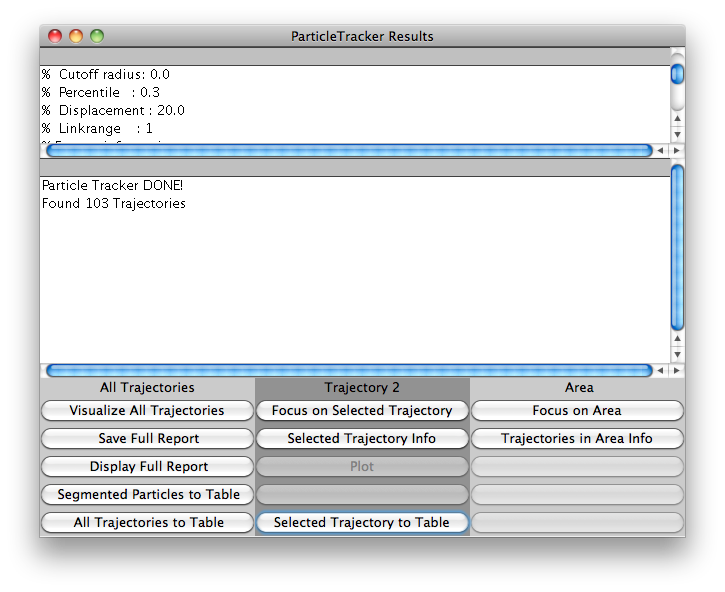
\includegraphics[scale=0.45]{fig/fig253_ParticleTrackerResults.png}
\caption{ParticleTracking Results}
\label{fig:particletrackingresults}
\end{center}
\end{figure}
In there, it should be reported that over 100 trajectories were detected. You could see how they look like by clicking "Visualize All Trajectories". 
Another window overlaid with colorful tracks appears 
(Fig. \ref{fig:particletrackingTracks}). 
Click "Filter Options" and input 10, so that short trajectories become invisible in the window. 
Use your mouse and select one of trajectory by clicking. 
Rectangle ROI is created in the surrounding of the selected track. 
Go back to the Results window (Fig. \ref{fig:particletrackingresults}) 
and click "Focus on Selected Trajectory". 
Then you will see another window is created with only the track you chose 
(Fig. \ref{fig:particletrackingTrackFocused}). 
Check carefully if the tracking was done properly. 
If you are satisfied, go back to the result window (Fig. \ref{fig:particletrackingresults}) 
again then click "selected trajectory to Table". 
You will then find the trajectory data is transferred to the Results table of ImageJ 
(Fig. \ref{fig:particletrackingTransferred}). 
 

%double figure
\begin{figure}[htbp]
 \centering
 \subfloat[]{\label{fig:particletrackingTracks}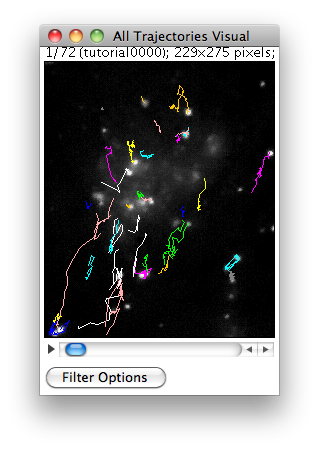
\includegraphics[height = 90mm]{fig/fig253particletrackingTracks.png}}
 \subfloat[]{\label{fig:particletrackingTrackFocused}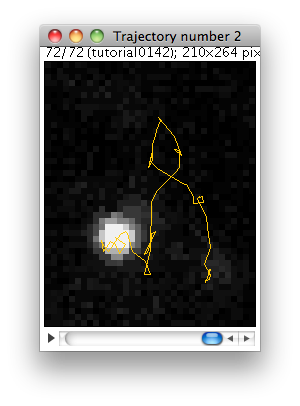
\includegraphics[height = 90mm]{fig/fig253_focusedTrajectory.png}}
 \caption{ (a) ParticleTracking Trajectories, all, and (b) Focus on Single Track.}
 \label{fig:particletrackingTrackFocused}
\end{figure}

 %figure 
\begin{figure}[htbp]
\begin{center}
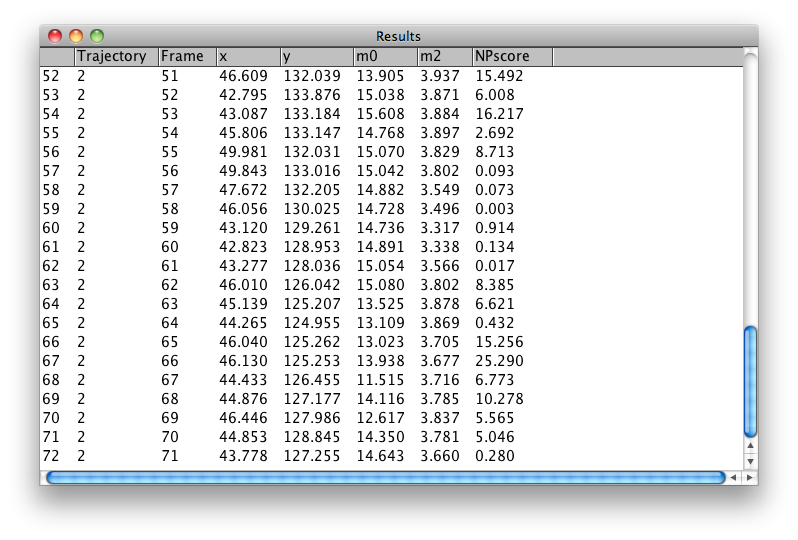
\includegraphics[scale=0.4]{fig/fig253_TrackingResultsInResultsTabel.png}
\caption{ParticleTracking Results transferred to ImageJ Results Table}
\label{fig:particletrackingTransferred}
\end{center}
\end{figure}

So now, what we have to do is access results table, 
get XY coordinates from there and do intensity measurements at corresponding positions. 
To get data out of results table, we use the following macro function:
\begin{indentCom}
\textbf{getResult("Column", row)}\\
Returns a measurement from the ImageJ results table or NaN if the specified column is not found. 
The first argument specifies a column in the table. 
It must be a "Results" window column label, such as "Area", "Mean" or "Circ.". 
The second argument specifies the row, where 0<=row<nResults. 
nResults is a predefined variable that contains the current measurement count. 
(Actually, it's a built-in function with the "()" optional.) 
Omit the second argument and the row defaults to nResults-1 (the last row in the results table). 
See also: nResults, setResult, isNaN, getResultLabel.
\end{indentCom}
Let's first test with a short macro that reads data from Results table and 
print out XY coordinates in the Log window. 

\lstinputlisting[morekeywords={*, getResult, nResults}]{code/code24.ijm}

At line 1, \ilcom{nResults} is a function that returns the number of rows in the Results table. 
Frame number is added with 1 in the line 2  because frame number in ParticleTracker plugin starts from 0, 
while it starts from 1 in ImageJ. 
In line 3 and 4, xpos and ypos is inverted, 
because ParticleTracker program was originally wrote in Matlab and for that convention 
(in Matlab, vertical diretion is called "X" and horizontal direction is called "Y", 
and this is common to matrix calculation software since row = X and column = Y), 
XY data should be inverted for use in in ImageJ. 

If you check the log window and if you are confident with data read out from Results window, 
we could now add the code with lines to measure intensity by 
placing circular ROI at XY coordinates of trajectory. Here we go. 

\lstinputlisting[morekeywords={*, getResult, makeOval}]{code/code24_5.ijm}

Running this macro, you should see a new column in Results window with header title "RoiInt", 
where measured intensity is listed (Fig. \ref{fig:PTResultsTableAfter}).

%figure 
\begin{figure}[htbp]
\begin{center}
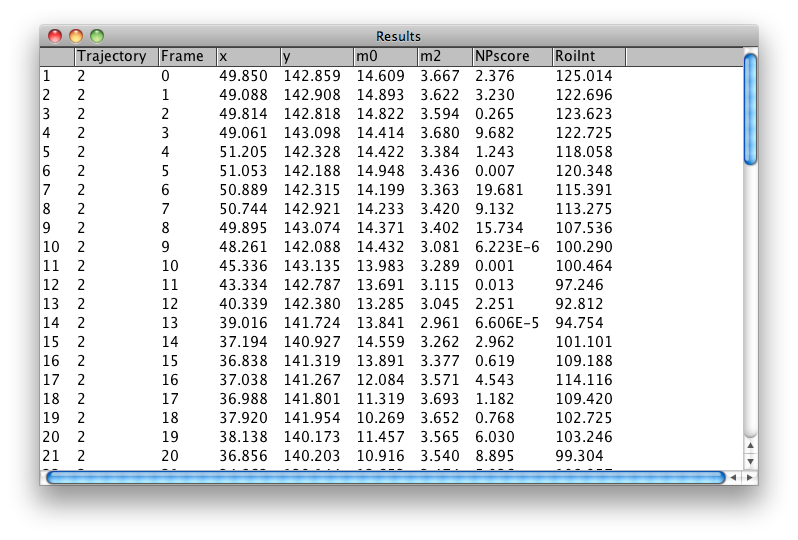
\includegraphics[scale=0.5]{fig/fig261_resultstableAddedWithInt.png}
\caption{Results Table with Intensity Measurement \\Column "RoiInt"}
\label{fig:PTResultsTableAfter}
\end{center}
\end{figure}

Explanation of the code: In the first line, 
we set the name of the image stack so that we are sure with which window to be measured with intensity. 
Line 2 and 3 are for setting the size of oval ROI. 

The way oval ROI is created is what you have learned already in detail in the section 
\ref{sec:dotmove}. \ilcom{getRawStatistics()} returns basic parameters of the selected ROI, 
and is more convenient than using \ilcom{run("Measure")}. 

\begin{indentCom}
\textbf{getRawStatistics(nPixels, mean, min, max, std, histogram)}\\
This function is similar to getStatistics except that the values returned 
are uncalibrated and the histogram of 16-bit images has a bin width of one and is returned 
as a max+1 element array. For examples, refer to the ShowStatistics macro set. 
See also: calibrate and List.setMeasurements
\end{indentCom} 

\subsection{Using values in non-Results table}
Next, we study a case when data are shown in non-Results Table. 
Manual Tracking plugin is another way of measuring particle movement, and utilizes non-Results table. 

\begin{indentexercise}{1}
Open sample image stack \textbf{TransportOfEndosomalVirus.tif} 
and track at least two virus manually\footnote{ For detailed instruction on how to use Manual tracker, 
see corresponding section in CMCI Image Processing and Analysis Course I Basic.}. 
In ImageJ, you should install this plugin by yourself. 
In Fiji, Manual Tracking plugin could be found at \ijmenu{[Plugins > tracking >]}.
\end{indentexercise}

After the tracking, we have a results table that looks like figure \ref{fig:manualtrackingresults}.
%figure 
\begin{figure}[htbp]
\begin{center}
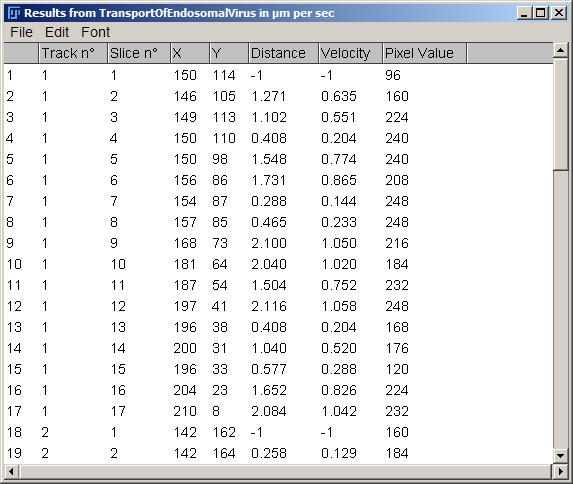
\includegraphics[scale=0.6]{fig/fig253_ManualTrackerResultsWindow.png}
\caption{Manual Tracking Results}
\label{fig:manualtrackingresults}
\end{center}
\end{figure}

To extract these data and use it for the secondary measurement, 
you might immediately think of using \ilcom{getResult(column header, row)} 
as we did in the previous subsection.

That should then be pretty straight forward\ldots 
But if you try this, you would see that this function returns error and 
does not work in case of Manual Tracking plugin. 
This is because result table created by Manual Tracking plugin is not the genuine ImageJ Results window. 
For such non-genuine results window, we retrieve data using the following function. 
\begin{indentCom}
\textbf{getInfo("window.contents")}\\
If the front window is a text window, returns the contents of that window. 
If the front window is an image, returns a string containing the text that would be displayed by 
Image>Show Info. Note that \ilcom{getImageInfo()} is a more reliable way to retrieve information 
about an image. Use \\
\ilcom{split(getInfo(),"\textbackslash{}n")} \\
to break the string returned by this function into separate lines. Replaces the \ilcom{getInfo()} function.
\end{indentCom}

This function returns a string with the content of the table. 
Try the following two lines to see how it works. \\

\begin{lstlisting}[numbers=none, morekeywords={*, getInfo}]
str = getInfo("window.contents");
print(str);
\end{lstlisting}
If you run these two lines, you will see data printed out in the Log window 
(Fig. \ref{fig:manualtrackingresultsLog}). 
%figure 
\begin{figure}[htbp]
\begin{center}
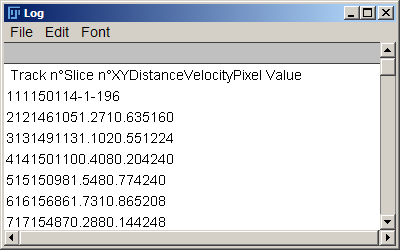
\includegraphics[scale=0.6]{fig/fig253_AllValuesinLog.png}
\caption{Manual Tracking Results in Log window}
\label{fig:manualtrackingresultsLog}
\end{center}
\end{figure}

So far so good, we succeeded in getting data out of the results table. 
Then what we need to do now is to play around with the \ilcom{str} variable, 
where all the data is now contained as a chunk. Since this chunk of data is not usable directly, 
we first split the \ilcom{str} to single lines of a string array. 
For this we use the \ilcom{split} function, the definition of which is 

\begin{indentCom}
\textbf{split(string, delimiters)}\\
Breaks a string into an array of substrings. 
Delimiters is a string containing one or more delimiter characters. 
The default delimiter set " \textbackslash{}t\textbackslash{}n\textbackslash{}r" 
(space, tab, newline, return) is used if delimiters is an empty string or split is called with only one argument. 
Returns a one element array if no delimiter is found. 
\end{indentCom}

Using this function to convert the string to a string array and adding two more lines to check the content of the array, 
the code now looks like this:\\
\begin{lstlisting}[numbers=none, morekeywords={*, split}]
str = getInfo("window.contents");
//print(str);
strA = split(str, "\n");
print(strA[0]);
print(strA[1]);
\end{lstlisting}
We use the delimiter \ilcom{\textbackslash{}n} which means "new line", a hidden character in \ilcom{str} 
that feeds a new line to form a table. When we run the above code we will see two lines of data shown in the log window (Fig. \ref{fig:splittedLine}).
%figure 
\begin{figure}[htbp]
\begin{center}
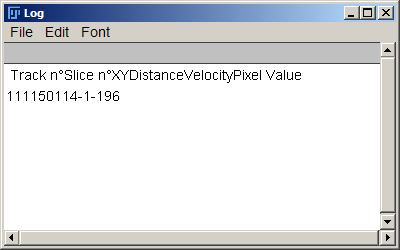
\includegraphics[scale=0.6]{fig/fig253_ZeroAndfirstlineValues.png}
\caption{Two Lines from data in the Log window}
\label{fig:splittedLine}
\end{center}
\end{figure}

We then still need to split each single line to individual data for each column. We modify the code as follows:
\begin{lstlisting}[numbers=none, morekeywords={*, split}]
str = getInfo("window.contents");
strA = split(str, "\n");
lineA = split(strA[1], "\t");
print(lineA[3]);
\end{lstlisting}

We use the delimiter \ilcom{\textbackslash{}t}, which means "tab", to convert a single line to an array of individual pieces of data (one element for each column). 
%figure 
\begin{figure}[htbp]
\begin{center}
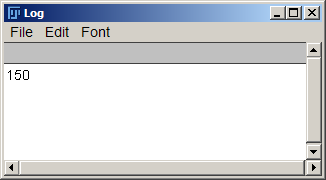
\includegraphics[scale=0.6]{fig/fig253_XfirstlineValue.png}
\caption{Elementary data in the Log window}
\label{fig:doublesplittedLine}
\end{center}
\end{figure}

The value shown in the Log window (Fig. \ref{fig:doublesplittedLine}) 
should be the same as the X value in the first row of the original table (Fig. \ref{fig:manualtrackingresults}). 

We now know how to access individual data values within \ilcom{str}, 
by first splitting it with delimiter \ilcom{\textbackslash{}n} and then by
\ilcom{\textbackslash{}t}. We can print all XY coordinates in the Log window with the following code.  

\lstinputlisting[morekeywords={*, split}]{code/code25.ijm}

If you encounter an error message with \ilcom{lineA[]} such as shown in fig.\ref{fig:fig262_ErrorMessage}, 
this is just because there is another text widow open and the \ilcom{getInfo()} function worked on 
that window rather than the results table of the Manual Tracking. To avoid such error, 
close the extra text windows and then try running the macro again. 
%figure  
\begin{figure}[htbp]
\begin{center}
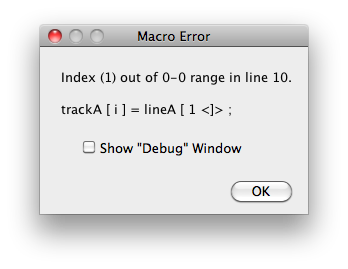
\includegraphics[scale=0.6]{fig/fig262_PossibleErrorMessage.png}
\caption{Possible Error Message with Code25 and Code25.5}
\label{fig:fig262_ErrorMessage}
\end{center}
\end{figure}

From line 4 to 7, new arrays are generated to store data from four columns in the for-loop from line 8 to 14. 

%figure  
\begin{figure}[htbp]
\begin{center}
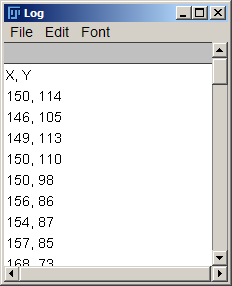
\includegraphics[scale=0.6]{fig/fig253_CoordinatesPrintedOut.png}
\caption{Elementary data in the Log window}
\label{fig:fig253_CoordinatesPrintedOut}
\end{center}
\end{figure}

Check the log window (Fig. \ref{fig:fig253_CoordinatesPrintedOut}), 
compare the output with the manual tracker results table, and if you are confident that you are accessing the right data in the table, 
you could then use the XY coordinates to place a circular ROI, 
measure the average intensity in that area and list them in the ImageJ Results window.

\lstinputlisting[morekeywords={*, split}]{code/code25_5.ijm}

Running this code, you should see a Results window that looks like figure 
\ref{fig:fig262_ManualTrackIntfinalResults}, tracking data plus measured intensity is shown in 
the column titled "RoiInt". The way the oval ROI is used to measure the mean intensity is similar to what 
we have coded in the previous subsection. A difference is that this time, we use arrays that store data 
extracted by splitting the chunk of string data. 

%figure  This should be replaced with results window!!!
\begin{figure}[htbp]
\begin{center}
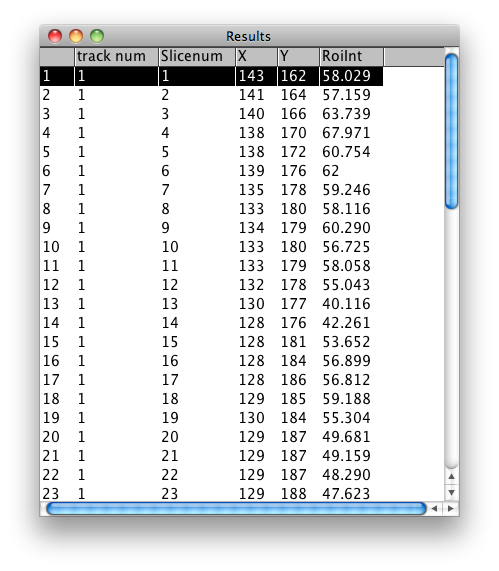
\includegraphics[scale=0.5]{fig/fig262_ManualTrackIntensityFinalResults.png}
\caption{ Manual Tracker Results in IJ Results table\\ now with measured intensity column RoiInt}
\label{fig:fig262_ManualTrackIntfinalResults}
\end{center}
\end{figure}

We then successfully measured the intensity dynamics of moving object again.  

\newpage
\subsection{Accessing Data File: Simple Case}
In this section and in the next section, 
we study how to access data in saved file for secondary measurements. 

Two cases we studied so far were both accessing data listed in a table that is already loaded in ImageJ 
(data is already an instance of ImageJ). What if we want to use data that is saved as a file? For example, 
we want to use results of Manual Tracking (previous section) that was saved as an .xls file and 
you want to use its data for secondary measurement. More generally, you did particle tracking using different software 
such as Imaris Track, and you want to use  coordinate data from that analysis for intensity measurement to be done in ImageJ. 
In such cases, we should access tabulated data in file accessing from ImageJ. 

In this section, we try accessing data saved by Manual Tracking. 
Loading data file could be done by a small modification 
of the code we studied in the previous section. Instead of the function 
\ilcom{getInfo("window.content")} in line 3 of code 25.5, we use \ilcom{FileOpenAsString(path)} to retrieve 
file content into a string variable.  By leaving the argument \ilcom{path} blank (""), user will be asked for choosing a file. 
Since this is a simple one-line replacement of line 3 of code 25.5, below is the new code but only showing its first 10 lines.  

\lstinputlisting[linerange={1-10}, morekeywords={*, File, openAsString}]{code/code26.ijm}

To run this macro, be sure that you have your stack already opened, as it is required for measuring intensity. 

\subsection{Accessing Data File: Complex Case}

We now try making use of data file with more complex format. 
In the case we studied with Manual Tracking plugin in the previous section, data format was pretty straight forward 
so we did not have to do much work for dealing with the data format. 
In general, things are not so simple and one must figure out some way to decode the format for using it in secondary measurement. 

Automatic tracking plugin "ParticelTracker" allows you to save trajectory data by "Save Full Report" 
button in the results interface (see Fig. \ref{fig:particletrackingresults}). 
We try to access this data. 
\footnote{ This technique is especially important if you want to do automated particle tracking of many data. 
A new feature in ParticleTracker plugin released in Nov. 2010 is that when ParticleTracker is called from macro, 
it automatically saves data in folder where the image file is located. We then are able to process many files using macro, 
even recursively, and get tracking data automatically. For this reason technique for accessing ParticleTracker data file is valuable.}

First, you must prepare the data file. 

\begin{indentexercise}{1}
\item Open sample image stack \textbf{TransportOfEndosomalVirus.tif}. 
Then do \ijmenu{[Plugins > Particle Detextor \& Tracker> Particle Tracker]}. 
An interface appears, so fill in the parameters as follows:
\begin{itemize}
\item radius: 3
\item cutoff: 0
\item percentile: 0.3
\item link range: 1
\item distance: 20
\end{itemize}
\item Click "Save Full Report" and save the data file in the folder where sample image stack 
"\textbf{TransportOfEndosomalVirus.tif}" is. 
Saving dialog will come up with a proposal of file name to be "Traj\_<filename>.txt" 
so do not change that and simply click Save (this file name will be important). 
Close the Results interface. Do not close the image stack \textbf{TransportOfEndosomalVirus.tif}, 
as we will use it still in the following.
\end{indentexercise}

Now you are ready with data, so we try loading data into ImageJ/Fiji. Run the following code. 

\lstinputlisting[morekeywords={*, substring, lengthOf,File, exists, openAsString}]{code/code27_PTfileaccess.ijm}

You now have all the values in the log window, that should look like fig. \ref{fig:fig264_PTdatainLogWin}. 

%figure  
\begin{figure}[htbp]
\begin{center}
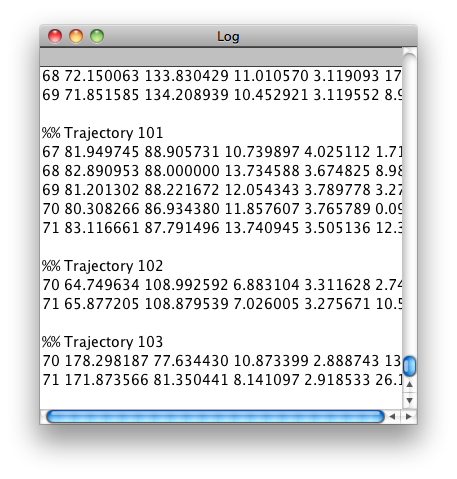
\includegraphics[scale=0.5]{fig/fig264_PTdataLoadedtoLog.png}
\caption{ ParticleTracker data loaded to Log Window}
\label{fig:fig264_PTdatainLogWin}
\end{center}
\end{figure}

Before getting into data file structure, let's look at what we have done in the code above. 
You might then study about how to deal with string, extracting parts of it. 
\begin{itemize}
\item Line 2: \ilcom{getDirectory} function with option \ilcom{("image")} 
will return a path of the last-opened image location. 
This will be where the file "\textbf{TransportOfEndosomalVirus.tif}", inside the sample image folder. 
\item Line 3: Filename of the image  "\textbf{TransportOfEndosomalVirus.tif}" is acquired. 
\item Line 4: Generating the file name of the data file. "Traj\_" is the prefix that was automatically added to 
the data file name. Function \ilcom{substring} extracts part of the string variable, and in our case, 
we try to get the image file name without ".tif". Definition of \ilcom{substring} function is as follows.

\begin{indentCom}
\textbf{substring(string, index1, index2)}\\
Returns a new string that is a substring of string. The substring begins at index1 and extends to the character at index2 - 1. 
See also: indexOf, startsWith, endsWith, replace.
\end{indentCom}

index1 should be 0, as we want from the beginning of the file name, and index2 should be 4 strings before the 
last string so we need the total length of the string. For this we use \ilcom{lengthOf} function. 
\begin{indentCom}
\textbf{lengthOf(str)}\\
Returns the length of a string or array.
\end{indentCom}
In this way, we construct the file name we want to access 
(the name of which originally is automatically generated when saving the data in Particle Tracker interface) 
the file further setting the full path to the file in line 5. 
\item Line 8: This line checks if the file full path generated above is valid. 
\ilcom{File.exists(full-path-to-file)} returns false if there is no such file. In that case, we should not proceed more so macro terminates at line 8. 
\item Line 11: If everything is ok, then the file is opened as a string, 
and the string will be printed in Log window by line 12. 
\end{itemize}

ParticleTracker data file consists of three parts. 
\begin{enumerate}
\item Header: contains information on the condition of tracking. 
\item Detected Particles: Detected particles in each frame is listed.
\item Trajectories: Trajectories are listed, one by one. 
\end{enumerate}
Since we need to access trajectory information, we need to go through the data string to reach the third part of the data structure. 
To do so we split the file by lines (\textbackslash{}n), then loop through the array to find the position where the trajectory information is contained. 

We examine the data file in detail, to see what could be the marker for the starting and end point of each trajectory. 
Here is a part of data, that is a directly copy and pasted below. 
\begin{lstlisting}[numbers=none]
24 154.894485 137.063614 7.338140 3.316167 15.683273
25 154.217377 138.368927 7.087145 3.417947 0.188002

%% Trajectory 37
15 22.111439 204.511826 9.726052 3.180977 28.252821
16 8.837964 209.618210 13.082743 3.273177 29.163294
17 0.432002 208.377045 3.574241 1.552869 0.000000
18 2.150804 209.609573 11.131773 2.939974 13.455443
19 10.542578 206.151169 14.173851 3.202391 14.258223
20 9.727753 206.960999 14.360144 3.250930 6.493425
21 15.708366 207.058640 14.943080 3.121640 0.053831
22 26.715679 208.680145 14.648912 3.091611 1.570746
23 29.143650 208.706314 13.616717 2.975144 21.279413
24 28.148304 202.200867 12.116886 2.862307 6.292521

%% Trajectory 38
15 142.326370 81.088326 5.813046 2.967546 13.995440
\end{lstlisting}
Single trajectory data start with a line with "\%\%Trajectory " plus numbering, and ends with a blank space. 
We use these information as markers for determining the location of trajectory data within file. Each line of data consists of 6 numbers: 
\begin{enumerate} 
\item Frame number
\item Y coordinate
\item X coordinate
\item image moment m0
\item image moment m2
\item Non-Particle Discrimination Criteria
\end{enumerate}
These values are separated by space. So splitting single line to an array of elementary data needs to be done by \ilcom{split(line, " ")}.

Here is a macro, that uses \ilcom{File.openAsString("")} to load the file and then loads the trajectory information 
into Results table with the strategy explained above. 

\lstinputlisting[morekeywords={*, }]{code/code28.ijm}

In the code 28, core of the processing resides within the function \ilcom{Load2ResultsV3}. 
It takes path to the data file and file name as arguments, and first opens the file as string at line 15. 
The chunk of string is then split by lines and for-loop starts to go through the array of lines (line 19). 

In every line in the array, if the line is a starting marker "\%\% Trajectory <number>" is tested (line 22) . 
If that is the case, then do-while loop is started, that loops until all the trajectory points are read out (line 24 to 41). 
While this trajectory read out is done, counter for the for-loop \ilcom{i} 
is also incremented that when the do-while loop ends (line 25), the for-loop starts again from the 
line after the data of that trajectory. Exit from do-loop occurs when blank line is found (line 42). 

Inside the do-while loop, space character is replaced with tab delimiter (line 26 to 32). 
This is required, since ImageJ results importing only recognized tab-delimited file as a table.  

There is a small adjustment by another function \ilcom{CommaEliminator} at line 32. 
This is required for removing comma character in some cases (this happens when the data file was opened and saved in excel or so). 
You probably do not need this line and function as we are using the data file directly after saving them. I left it in the code for your future usage. 

Just to be sure with data content, line 33 and 34 double-check that the line indeed contains several data. 
Line 35 to 38 writes trajectory ID, Frame number and XY coordinates into Results window by \ilcom{setResult} function.

\begin{indentexercise}{2}
\item Finally, we can combine several macros and functions we studied so far to make a new macro 
that loads the ParticleTracker data file to Results table, and read out intensity. 
This could be done by combining following codes, with a bit of modifications with each. 
\begin{itemize}
\item code 27 (check the current image stack name and loads its track data file as string)
\item code 28 (data in string format is converted to Result table)
\item code 24.5 (measure intensity according to coordinates in Results table)
\end{itemize}
Bits and pieces are already there. Please try completing a macro that loads track data file according 
to the title of the image stack that is already opened, place them in Results table, and then measure 
the intensity in corresponding frame and position in the image stack. 
\end{indentexercise}